\begin{figure}
  \resizebox{\columnwidth}{!}{%
    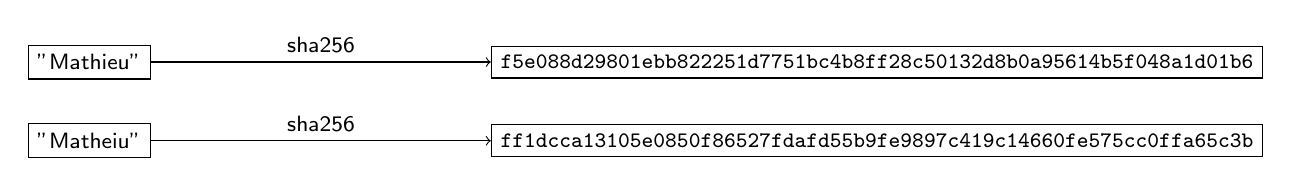
\begin{tikzpicture}[font=\sffamily\footnotesize,
        Input/.style={shape=rectangle,draw},
        Output/.style={shape=rectangle,draw}
      ]

      \node[Input] (I_1) at (0,0) {"Mathieu"};
      \node[Output] (O_1) at (10,0) {\texttt{f5e088d29801ebb822251d7751bc4b8ff28c50132d8b0a95614b5f048a1d01b6}};
      \node[Input] (I_2) at (0,-1) {"Matheiu"};
      \node[Output] (O_2) at (10,-1) {\texttt{ff1dcca13105e0850f86527fdafd55b9fe9897c419c14660fe575cc0ffa65c3b}};

      \draw[->] (I_1) -- (O_1) node[midway,above,sloped]{sha256};
      \draw[->] (I_2) -- (O_2) node[midway,above,sloped]{sha256};
    \end{tikzpicture}%
  }

  \caption{Sensibilité aux changements de la fonction SHA-256}
  \label{fig:sha256-hash-examples}
\end{figure}